\ifdefined\handoutmode
  \PassOptionsToClass{handout}{beamer}
\fi
\documentclass[aspectratio=169]{beamer}

\input{../../../../hh_bpa_forel-preamble} % this is ugly.

\title{FMTS mätteknik HT2026 -- Dag 4}
\author{Pererik Andreasson \\ Struan Gray }
\date{\today{}}

\begin{document}

%%% Title slide: different footer, large logo
{
% no page #, no logo on title page
\setbeamertemplate{footline}{}
\setbeamertemplate{logo}{\titlelogos}
\begin{frame}
\vfill
  \begin{block}
    \maketitle
  \end{block}
\end{frame}
}


\frame{
    \frametitle{Lärandemål}
    {\Huge
    \begin{enumerate}
        \item<1-> Ensam mätning inget värt.
        \item<2-> Okalibrerat mätinstrument inget värt.
        \item<3-> Elektriska mätningar \emph{påverkar} mätobjektet $\rightarrow$ behöver \emph{tolkas}.
    \end{enumerate}
    }
}


\mode<beamer>{
\frame{
    \frametitle{Dagens plan}
    {\LARGE
        \begin{itemize}
            \item Fullvågslikriktare.
            \item Tidskonstant med oscilloskop.
            \item Filter med oscilloskop.
            \item Justera oscilloskopproben!.
            \item Induktor.
            \item Resonans.
        \end{itemize}
    }
    }   
} % end mode


\begin{frame}
\frametitle{\alert{Idag:} OBS större $U_{PP}$ (tänk procent)}
\resizebox{0.8\textwidth}{!}{%
\centering
  \begin{circuitikz}[american] 
  	\draw (0, 0)  
    to[sinusoidal voltage source, invert, l={$U_{PP}=\qty{20}{\V}$}, *-] (0,2)
    to[diode] (2, 2)
    to[R=$R$] (2, 0)
	-- (0, 0)
    node[ground, rotate=-90]{}
    ;
    \draw (2, 2)
    to[short,*-] (4, 2)
    to[oscope] (4, 0)
    to[short, -*] (2, 0) 
    ;
  \end{circuitikz}
} % end resizebox
\\\vspace{3mm}
\centering
{\LARGE  
 Hur ser spänningen över motståndet ut?
}% end LARGE
\end{frame}


\handoutnoteslide


\mode<beamer>{
\frame{
    \frametitle{}
    \begin{tikzpicture}[remember picture,overlay]
        \node[at=(current page.center)] {
            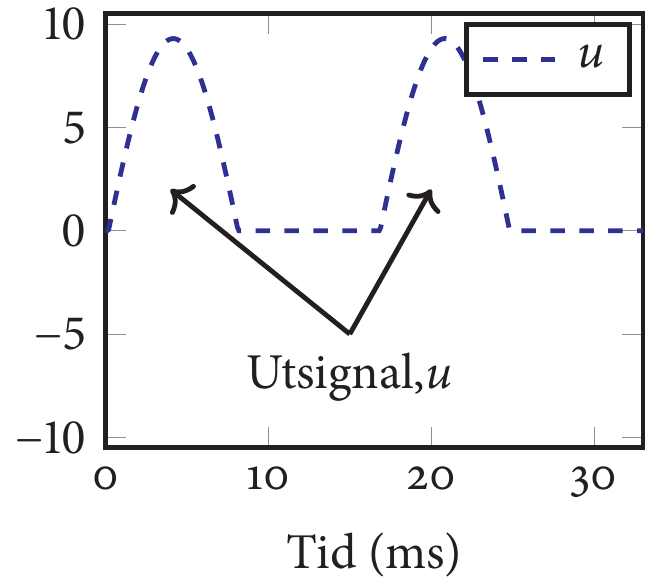
\includegraphics[keepaspectratio,
                                 width=\paperwidth,
                                 height=\paperheight]{figures/diod_svaret.png}
            };
    \end{tikzpicture}    
  }
}

\frame{
\frametitle{}
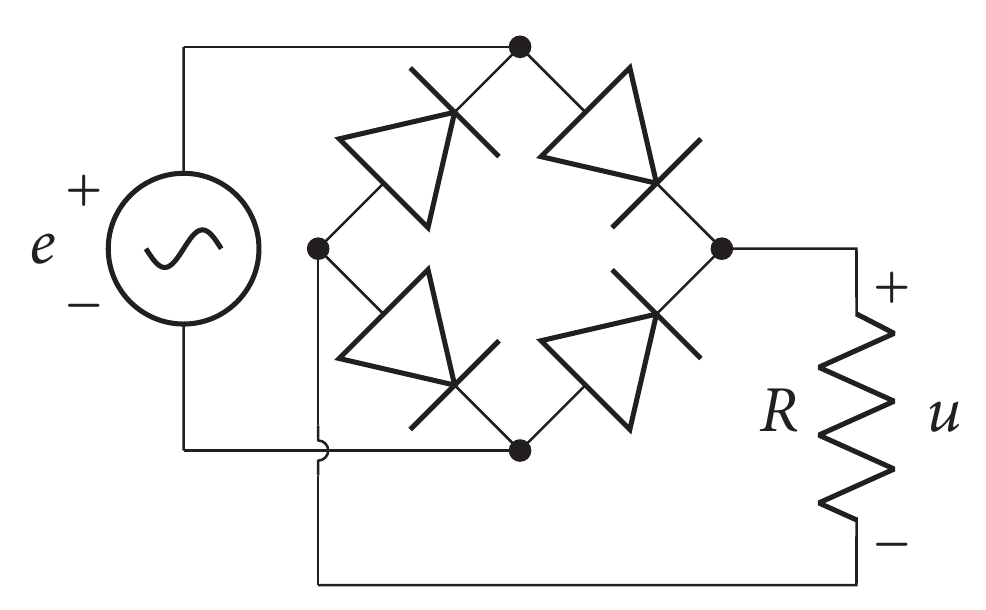
\includegraphics[width=\textwidth]{figures/likriktare.png}
}

\handoutnoteslide

\mode<beamer>{
\frame{
\frametitle{}\centering
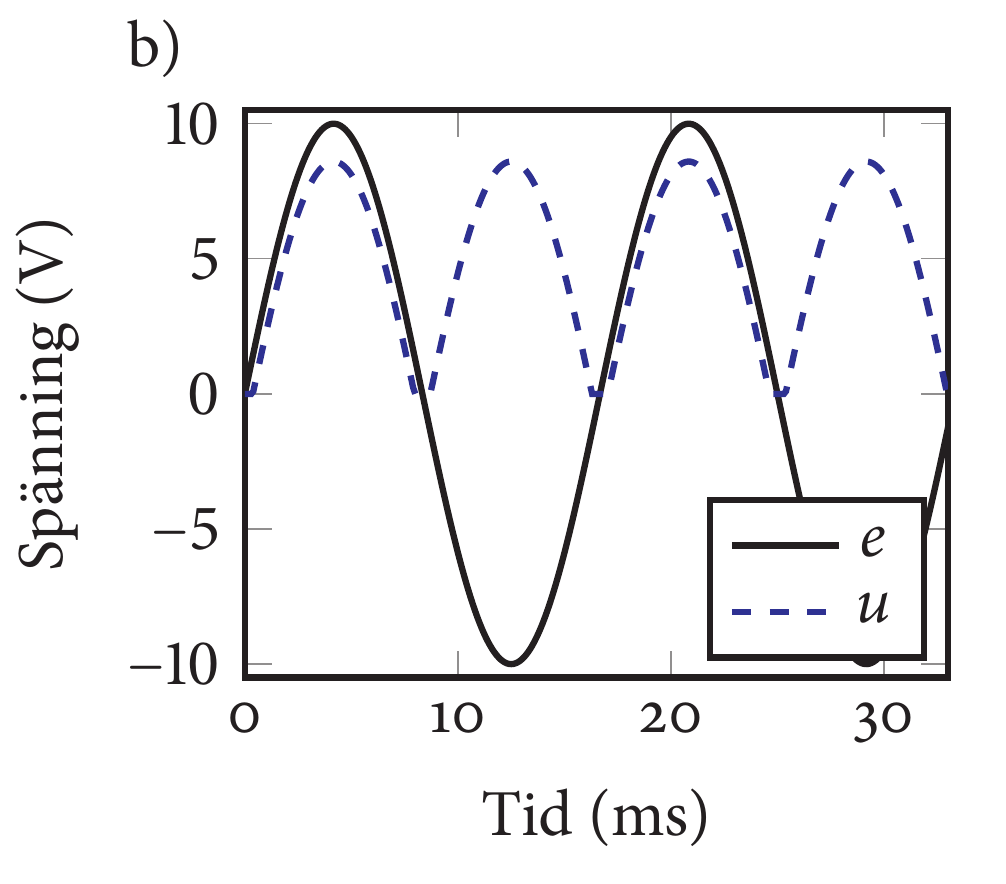
\includegraphics[width=0.7\textwidth]{figures/likriktare_svaret.png}
}
} 

\frame{
\frametitle{}
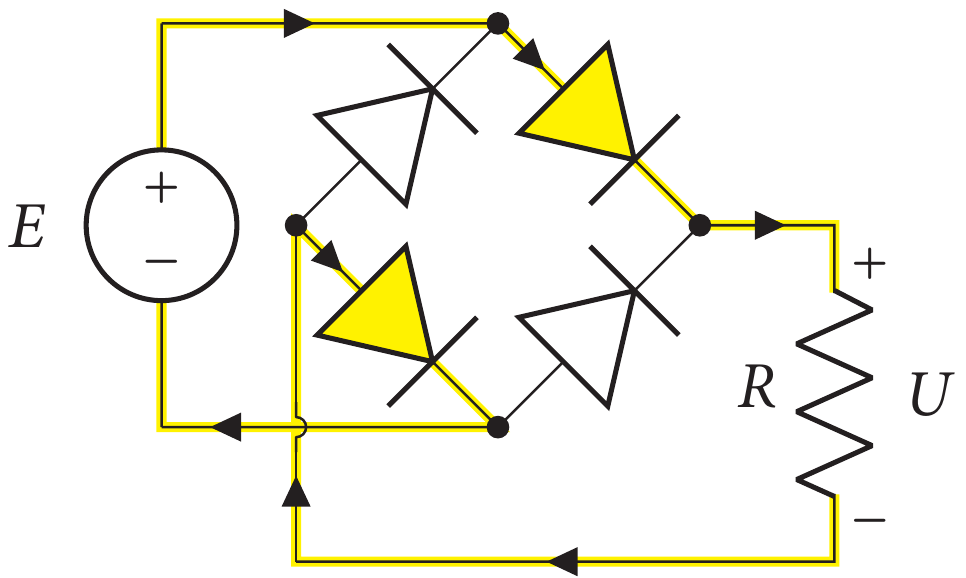
\includegraphics[width=\textwidth]{figures/likriktare_positiv.png}
}

\frame{
\frametitle{}
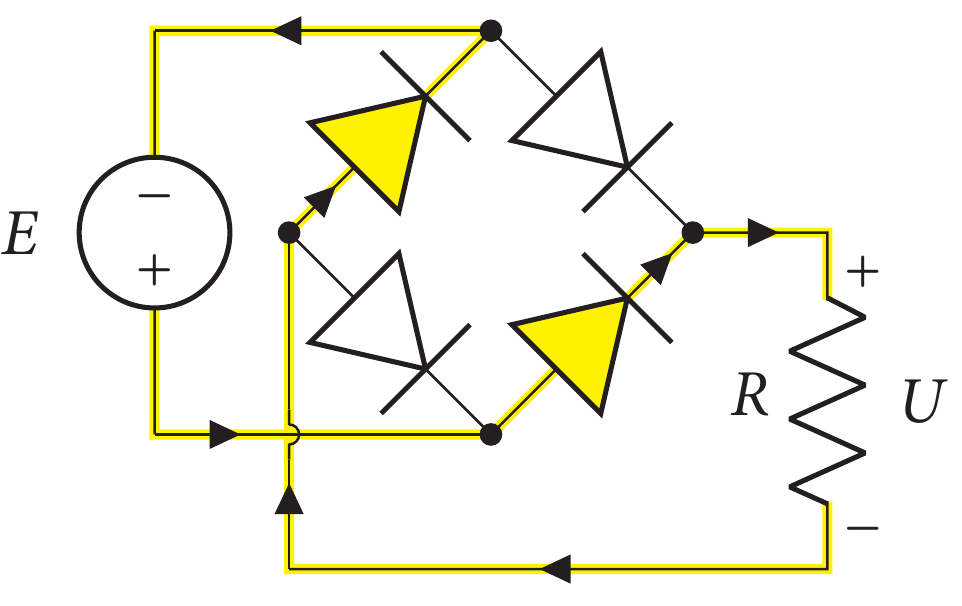
\includegraphics[width=\textwidth]{figures/likriktare_negativ.png}
}

\frame{
\frametitle{}
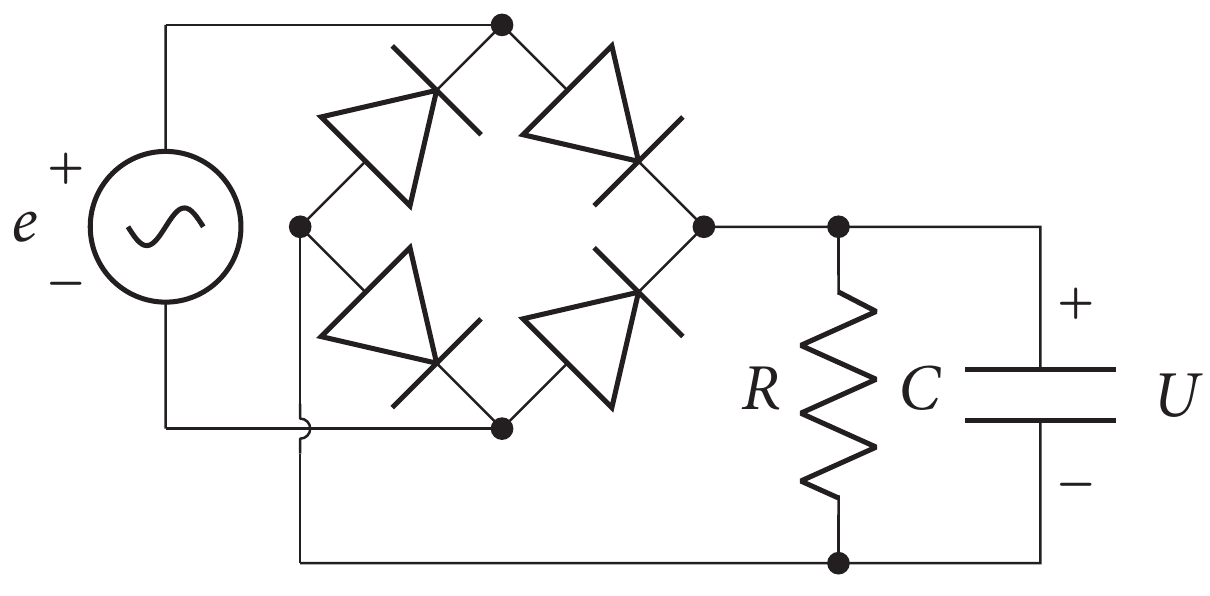
\includegraphics[width=\textwidth]{figures/likriktare_glattad.png}
}

\handoutnoteslide

\mode<beamer>{
\frame{
\frametitle{}\centering
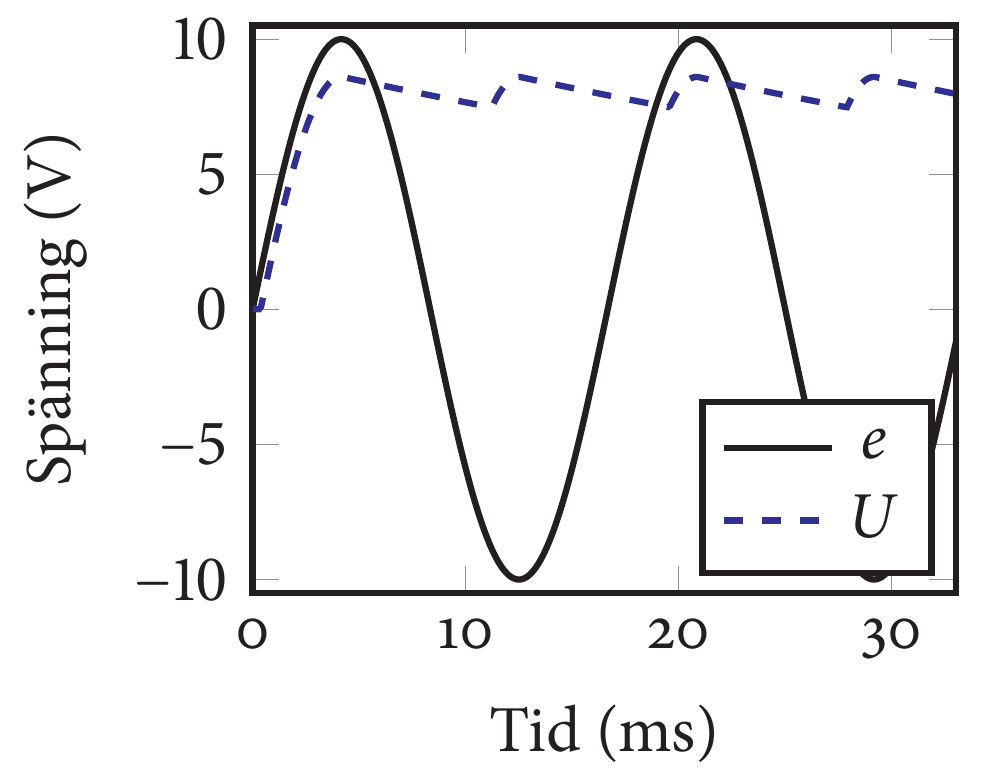
\includegraphics[width=0.7\textwidth]{figures/likriktare_glattad_svaret.png}
}
}


% mäta tidskonstant med oscilloskop.
% HT2026: när denna gjordes upptäcktes det att probarna var felinställda. 
% Då körde jag mätprobskalibreringsbilderna (kommer efter denna, är ripoff på emils.)
\begin{frame}
\frametitle{Kondensator och oscilloskop}
{\Large $C=\qty{13.3}{\nano\farad}$, $R=\qty{1}{\kilo\ohm}$ och $\hat{u}=\qty{2}{\V}$. Använd fyrkantspuler $f=\qty{1}{\kHz}$ och mät upp tidskonstanten (\qty{63}{\percent} av ändringen).}\\\vspace{3mm}
\resizebox{0.75\textwidth}{!}{%
\centering
\begin{tikzpicture}
    \ctikzset{bipoles/oscope/width=1.6}\ctikzset{bipoles/oscope/height=1.2}
    \node[oscopeshape, rotate = -90, rotated instruments](O)at(5,1){};
    \draw (O.in 1) to[short, *-] ++(-2.25,0) node[currarrow, 
    rotate=180]{};
    \draw (O.in 2) to[short, *-] ++(-1,0) to[short] ++ (0, -0.5) node[ground]{};
      	\draw (0, 0)  
    to[sinusoidal voltage source, invert, l={$U_{PP}=\qty{5}{\V}$}, *-] (0,2)
    to[R=\qty{1}{\kilo\ohm}] (2, 2)
    to[C=\qty{13.3}{\nano\farad}] (2, 0)
	  -- (0, 0) node[ground, rotate=-90]{} ;
\end{tikzpicture}
}\\[2mm]
{\Large Jämför med uträknade värden.}
\end{frame}


\handoutnoteslide

\descriptionslide{figures/probkalibrerin01.png}{}{}{}
\descriptionslide{figures/probkalibrerin02.png}{}{}{}
\descriptionslide{figures/probkalibrerin03.png}{}{}{}



\begin{frame}
\frametitle{Kondensator och oscilloskop 2 -- filter}
\resizebox{0.8\textwidth}{!}{%
\begin{tikzpicture}
    \ctikzset{bipoles/oscope/width=1.6}\ctikzset{bipoles/oscope/height=1.2}
    \node[oscopeshape, rotate = -90, rotated instruments](O)at(5,1){};
    \draw (O.in 1) to[short, *-] ++(-2.25,0) node[currarrow, 
    rotate=180]{};
    \draw (O.in 2) to[short, *-] ++(-1,0) to[short] ++ (0, -0.5) node[ground]{};
      	\draw (0, 0)  
    to[sinusoidal voltage source, invert, l={$U_{PP}=\qty{5}{\V}$}, *-] (0,2)
    to[R=\qty{1}{\kilo\ohm}] (2, 2)
    to[C=\qty{13.3}{\nano\farad}] (2, 0)
	  -- (0, 0) node[ground, rotate=-90]{} ;
\end{tikzpicture}
}\\\vspace{3mm}
{\Large Mät upp amplituden över kondensatorn för frekvenserna \qty{10}{\Hz}, \qty{100}{\Hz}, \qty{1000}{\Hz}, \qty{10000}{\Hz} och \qty{100000}{\Hz}. Skriv upp värdena i en tabell och rita upp en tydlig graf.}
\end{frame}

\handoutnoteslide

\mode<handout>{
\begin{frame}[plain]
    \centering
    \begin{tikzpicture}
        \begin{axis}[
            width=0.97\paperwidth,
            height=0.94\paperheight,
            anchor=center,
            scale only axis=false,
            xmin=0, xmax=10,
            ymin=0, ymax=6,
            axis lines=left,
            axis line style={->},
            xtick={0,1,...,10},
            ytick={0,1,...,6},
            xticklabels=\empty,
            yticklabels=\empty,
            tick style={draw=none},
            grid=major,
            major grid style={gray!40, thin},
            enlargelimits=false,
        ]
        \end{axis}
    \end{tikzpicture}
\end{frame}
} % end mode

\handoutnoteslide



\begin{frame}{A simple AM radio receiver}
    \vspace{-5mm}    
    \centering
        \begin{circuitikz}[transform shape]
            % Antenna input and coupling capacitor
            \draw
                (0,2) node[left]{Antenna}
                to[C, l=$C_{\mathrm{in}}$] (1.5,2)
                -- (4.2,2)
                to[D, l=$D_1$] (5.4,2)
                -- (8,2) node[right]{Audio};

            % Tuned circuit: parallel LC
            \draw (2.4,2) to[L, l_=$L$, *-*] (2.4,0);
            \draw (3.4,2) to[C, l=$C_{\mathrm{t}}$, *-*] (3.4,0);

            % Detector load and smoothing capacitor
            \draw (5.8,2) to[R, l=$R_{\mathrm{L}}$, *-*] (5.8,0);
            \draw (7,2) to[C, l=$C_{\mathrm{L}}$, *-] (7,0);

            % Common return
            \draw (2.4,0) -- (7,0);
            \draw (2.4,0) node[ground, rotate=-90]{};
        \end{circuitikz}

  \begin{columns}[c,onlytextwidth]
    \begin{column}{0.53\textwidth}
\begin{itemize}
              \item The diode rectifies the selected RF signal.
            \item $C_{\mathrm{L}}$ smooths the RF pulses; their changing
                  envelope follows the audio.
            \item $R_{\mathrm{L}}$ provides a discharge path. The audio
                  voltage is taken across the load.

\end{itemize}
    \end{column}

    \begin{column}{0.43\textwidth}
        \begin{itemize}
            \item The antenna picks up many AM stations.
            \item The $LC$ circuit is tuned to one station:
                  \[
                      f_0 \approx \frac{1}{2\pi\sqrt{LC_\text{t}}}
                  \]
        \end{itemize}
    \end{column}
\end{columns}
\end{frame}


%%--------------------------------------------------
%% Ny frame
%%--------------------------------------------------
\begin{frame}[fragile]{Växelström - Induktorn}
	\begin{columns}
		\column{0.3\textwidth}
			\alert{Växelström}
			$$i(t) = \hat{i}\sin\omega{}t$$
			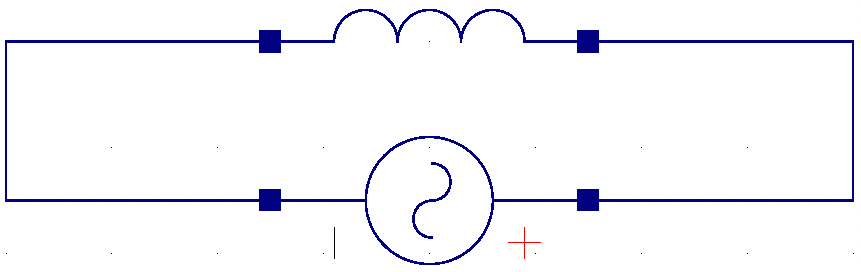
\includegraphics[width=\textwidth]{figures/UL.png}	\\
			                \onslide<3->{Strömmen går \SI{90}{\degree} \emph{efter} spänningen.\\}
        \onslide<4->{Ohms lag $U=\omega L\cdot{} I$ \alert{gäller bara för} effektivvärden och amplituder.}

		\column{0.7\textwidth}<2->
			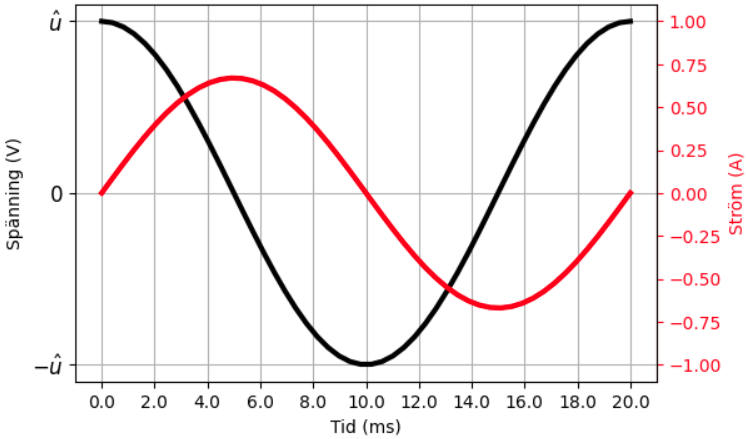
\includegraphics[width=\textwidth]{figures/IV_L.png}
	\end{columns}
	\vspace{5mm}
	\begin{center}
	\onslide<5->{
		$\omega L$ induktiva \alert{reaktansen} $X_L$ (\unit{\ohm})
	}
	\end{center}
\end{frame}

\handoutnoteslide

%%--------------------------------------------------
%% Ny frame
%%--------------------------------------------------
\begin{frame}[fragile]{Växelström - Induktorn}

	{\LARGE
	En spole har reaktansen \qty{160}{\ohm} vid \qty{1}{\kHz}. Beräkna dess reaktans
	vid \qty{25}{\Hz}.
	}
	\vspace{30mm}
\end{frame}

\handoutnoteslide

\begin{frame}{We are doing it! New component!}
Spole mellan 0,1 – 10 mH. Välj $R = \qty{1}{\kilo\ohm}$.   Beräkna frekvensen enligt $f=\frac{R}{2\pi L}$ 
   \begin{center}
%  \includegraphics[width = 0.75\textwidth]{figures/ACspole.png}
\resizebox{0.6\textwidth}{!}{
\begin{tikzpicture}[american]
	\draw (0, 0) node[ground] {} to[sV=, *-, v<={$V_\text{AC}$}] (0, 3.5)
		to[short] (2, 3.5)
		to[L=$L$, v=$U_{L}$] (2, 1.75)
		to[R=$R$, v=$U_{R}$] (2, 0)
		to[short] (0, 0)
		;
\end{tikzpicture}\hspace{10mm}\onslide<2->{
\begin{tikzpicture}
	\draw[->] (0, 0) -- (0:3cm) node[anchor=west] {Re};
	\draw[->] (0, 0) -- (90:3cm) node[anchor=south] {Im};
	\draw[-{Straight Barb}, ultra thick, blue] (0, 0) -- (90:2cm) node[anchor=south west] {$U_{L}$} ;
	\draw[-{Straight Barb}, ultra thick, red] (0, 0) -- (0:2cm) node[anchor=south west] {$U_{R}$} ;
	\draw[-{Straight Barb}, ultra thick] (0, 0) -- (45:2.83cm) node[anchor=south west] {$U_{R}+U_{L}$} ;
	\draw[dashed] (-0.2, 2) -- (2.2, 2) ;
	\draw[dashed] (2, -0.2) -- (2, 2.2) ;
	\draw[->, gray, thick] (10mm,0) arc [start angle=0, end angle=45, radius=10mm] node[anchor=north west, xshift=2mm, yshift=0mm] {$\varphi$};
\end{tikzpicture} } % onslide
} % resizebox

Oscilloskopa mellan komponenterna och över hela. Bestäm spänningarna och fasvinkeln.
\end{center}
\end{frame}

\handoutnoteslide

% Resonance circuit.
% Slide 1: setup
\begin{frame}{Series RLC resonance: setup}
\centering
\begin{circuitikz}[scale=0.9, transform shape]
    % Series circuit
    \draw
        (0,0) node[ground]{}
        to[sV, l={$U_{PP}$=\qty{2}{\V}}] (0,3)
        to[L, l=$10\,\mathrm{mH}$] (2,3)
        to[C, l=$22\,\mathrm{nF}$] (4,3)
        to[R, l=$220\,\Omega$] (4,0)
        -- (0,0);

    % Oscilloscope connections across the resistor
    \draw[blue, dashed, thick]
        (4,3) -- (5.5,3.5) -- (7,3.5);
    \draw[blue, dashed, thick]
        (4,0) -- (5.5,2.0) -- (7,2.0);

    % Simple oscilloscope symbol
    \draw[thick] (7,1.8) rectangle (9.5,3.7);
    \draw[thick] (7.5,2.35) rectangle (9.0,3.25);
    \draw[blue, thick]
        (7.65,2.8) -- (7.9,2.8) -- (8.1,3.05)
        -- (8.35,2.55) -- (8.6,2.8) -- (8.85,2.8);
    \node at (8.25,3.5) {Oscilloscope};
    \node[blue, right] at (9.05,3.5) {CH1 tip};
    \node[blue, right] at (9.05,2.0) {CH1 ground};
\end{circuitikz}

\vspace{0.4em}

Svep generatorfrekvensen och observera spänningen över motståndet. Börja på 1 kHz och öka upp till 20 kHz. Notera frekvensen där spänningen är som högst. Då $V_R$ är som högst, mät spänningen över spolen och kondensatorn. Notera även fasvinkeln mellan spänningen över motståndet och generatorn.
\end{frame}

\handoutnoteslide

\mode<beamer>{
% Slide 2: what to observe
\begin{frame}{Sweep the frequency}
\centering
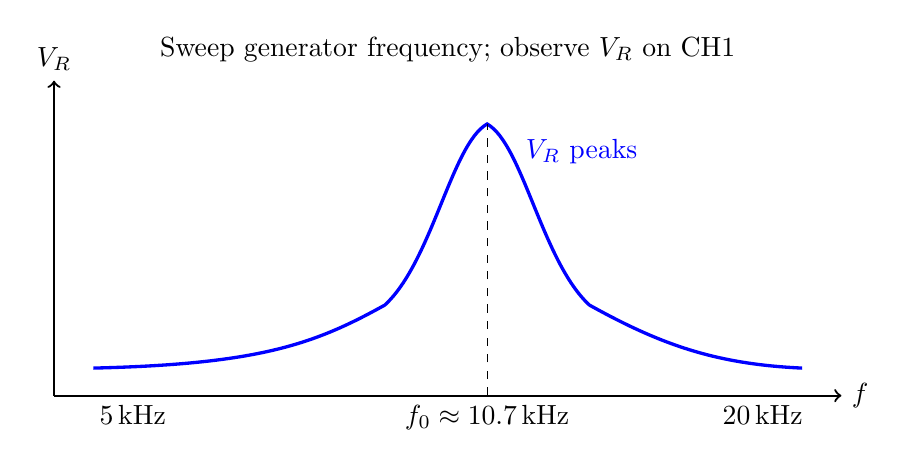
\begin{tikzpicture}[x=1cm,y=1cm]
    % Axes
    \draw[->, thick] (0,0) -- (10,0) node[right] {$f$};
    \draw[->, thick] (0,0) -- (0,4) node[above] {$V_R$};

    % Illustrative response
    \draw[blue, very thick]
        (0.5,0.35)
        .. controls (2.6,0.4) and (3.3,0.65) ..
        (4.2,1.15)
        .. controls (4.8,1.7) and (5.05,3.2) ..
        (5.5,3.45)
        .. controls (5.95,3.2) and (6.2,1.7) ..
        (6.8,1.15)
        .. controls (7.7,0.65) and (8.4,0.4) ..
        (9.5,0.35);

    % Resonance marker
    \draw[dashed] (5.5,0) -- (5.5,3.45);
    \node[below] at (5.5,0) {$f_0 \approx 10.7\,\mathrm{kHz}$};
    \node[blue] at (6.7,3.1) {$V_R$ peaks};

    % Sweep range labels
    \node[below] at (1,0) {$5\,\mathrm{kHz}$};
    \node[below] at (9,0) {$20\,\mathrm{kHz}$};
    \node[align=center] at (5,4.4) {Sweep generator frequency; observe $V_R$ on CH1};
\end{tikzpicture}

\vspace{0.6em}
At resonance: \qquad $X_L = X_C$
\end{frame}
} % end mode


\mode<handout>{
\begin{frame}[plain]
    \centering
    \begin{tikzpicture}
        \begin{axis}[
            width=0.97\paperwidth,
            height=0.94\paperheight,
            anchor=center,
            scale only axis=false,
            xmin=0, xmax=10,
            ymin=0, ymax=6,
            axis lines=left,
            axis line style={->},
            xtick={0,1,...,10},
            ytick={0,1,...,6},
            xticklabels=\empty,
            yticklabels=\empty,
            tick style={draw=none},
            grid=major,
            major grid style={gray!40, thin},
            enlargelimits=false,
        ]
        \end{axis}
    \end{tikzpicture}
\end{frame}
} % end mode

\handoutnoteslide



\mode<beamer>{\finalslide}

\end{document}
